\documentclass{article}
\usepackage[utf8]{inputenc}
\usepackage{graphicx}
\usepackage{float}

\title{Requirement Analysis and Specification Document: bike4share}
\author{Maffioli Sara, Papale Lorenzo, \\ Stucchi Lorenzo \& Vaghi Federica}


\begin{document}

\maketitle
\tableofcontents

\newpage

\section{Introduction}
\subsection{Purpose}
The aim of the project is to develop a web application called “bike4share” for a bike sharing service in order to guarantee to the user a web service to search for the availability of bikes and free stalls around his position or the desired location in the city.\\The web application must ensure the technician to have a private section showing analytic graphs and statistics on the bike flow in real time.
\subsection{Scope}
The “bike4share” application must provide a service of registration and of log-in both for user and technician.\\The user can access to some information related to availability and location of the stall which are shown by a web map, one of main functionalities of “bike4share”.\\The user can access to premium functions through the registration on web service, for example the mean of the available bikes and stalls in a certain hour that can be selected and a mail service to ensure the recovery of the forgot password.\\
“bike4share” must provide to the technician a dedicated analytic section, in order to analyse and study the bike stations trends in real time and also during a set span of time.\\This analytic section guarantees statistic, like mean of bikes used during a certain period and graphs showing trends, relying on the data stored in a designed database.
\subsection{Definitions, acronyms, abbreviations}
DB:database\\
DBMS: database management system\\
b4s: bike4share\\
HW: hardware\\
SW: software\\
RASD: requirement analysis and specification document
\subsection{Reference documents}
the following documents are taken as reference for the developing of the b4s web application:
\begin{itemize}
    \item SE4G Lab assignment:GreatBikes given by Prof.ssa Elisabetta Di Nitto, PhD Eng. Daniele Oxoli
    \item Flask Web Developement -developing web application with Python- written by Miguel Grinberg
    \item Hands-On Data Visualization with Bokeh written by Kevin Jolly 
\end{itemize}


\subsection{Overview}
The RASD document is structured in four main chapters, i.e. Introduction, Overall Description, Specific Requirements and Appendices. 

\section{Overall Description}
This chapter is divided in five subchapters that are devoted to the description of the external interfaces and shared phenomena, summary of the major product functions, user characteristics, constraints and last one devoted to assumptions and dependencies.
\subsection{Product perspective}
The “b4s”application will work thanks to several components supporting it.\\ As shown in the scheme in Figure \ref{fig:schema}, it is possible to recognise three levels of the system: Data, Software and User.\\ 
Data are retrieved as input from the Databases.
Software is retrieved as output of Map and statistics visualisation.\\
User level makes possible to view the map and to obtain some information (from the user point of view) and the technician can perform API request to analyse data and statistics.\\ Both the actors can perform their purposes accessing the page through the browser.\\

\begin{figure}[h]
    \centering
    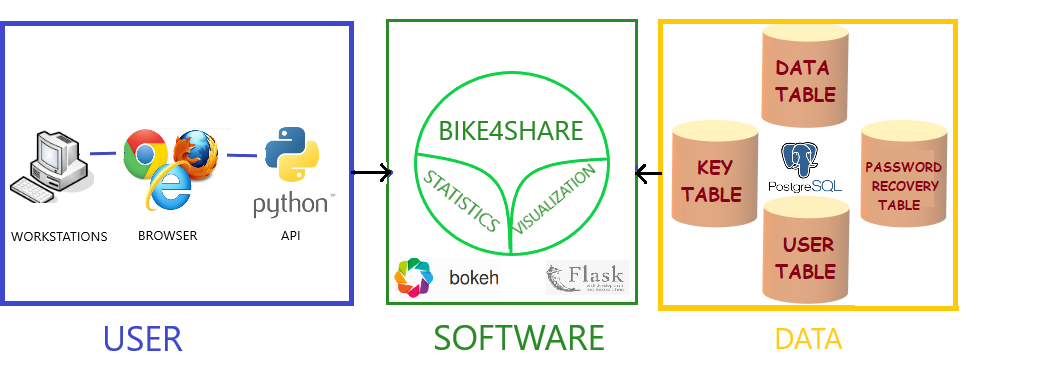
\includegraphics[width=0.75\linewidth]{image/BIKE4SHARE_SCHEMA_FINAL.png}
    \caption{Overall view of "bike4share" system}
    \label{fig:schema}
\end{figure}
The Venn diagram in figure \ref{fig:venn} shows a representation of the phenomena, world, shared and machine,  concerning the software.\\
\begin{figure}[h]
    \centering
    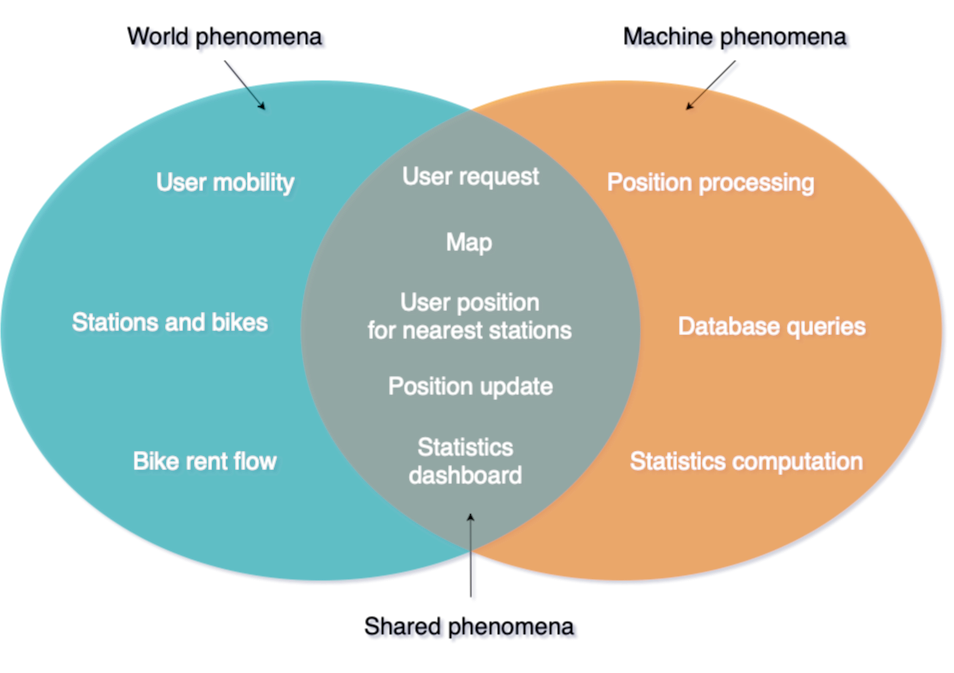
\includegraphics[width=0.75\linewidth]{image/venn.png}
    \caption{Venn diagram of the phenomena}
    \label{fig:venn}
\end{figure}\\\\

\subsection{Product functions}
"b4s” provides different functions to different type of users.\\
Basic functions are accessible to all the users and they consist in a web page with a map where the position and the total number of the stalls are shown for all the bike stations.\\
Premium functions are accessible to the registered users and they consists in the displaying of the position of the user on the map in order to help the detection of the nearest station.\\
A list of all the stations near the user's positions is also provided and it is shown in correspondence of the maps.\\
In case that the users won’t allow the access to their position or this feature won't be available for their systems,it could be possible to manually insert the address or select the position on the map.\\
A specific section of the application is been devoted to the technician’s use.\\
In order to access the technician is requested to complete the registration through a specific secret key that allows the first authentication, after that it's possible to log-in and to access at this specific section where instruments and graphical statistic tools are provided. 
\begin{itemize}
    \item Trend of the bikes usage during a selected span of time;
    \item Average of the bikes during the day, week or month
    \item The most used bike stalls shown as histogram during the day, week or month
    \item Real-time statistics of the bikes usage during the last day,week or month
    \item Total bikes availability per day of the week or month
    
\end{itemize}

\subsection{User characteristics}
\begin{itemize}
    \item \textbf{Registered user}: a user that is registered yet and that wants to access the “b4s” WebApp services in order to use the Premium Functions available on the application, it could be a person that uses this service frequently. 
    \item \textbf{Not registered user}: a user that isn’t registered yet and that wants to access the “b4s” WebApp  services in order to use the Basic Functions.\\ It could be a person that  doesn’t use this service frequently or a new user that wants to try it for the first time.
    \item \textbf{Technician}: a person who is authenticated thanks to specific credential given by the master of the service and  who has been granted supervising permissions; the technician is allowed to view, analyse, access statistics and aggregated information about the “bike4share” WebApp services.
\end{itemize}

\subsection{Constraints}
"b4s" WebApp has to respect different kind of constraints, it this session they will be briefly introduced.
\subsubsection{Regulatory Policies}
“b4s” relies on map applications as OpenStreetMap, Mapbox Satellite and Mapbox Street so it must respect their market policies.

\subsubsection{Interfaces to other applications}
“bike4share” interacts with different applications
\begin{itemize}
    \item Database Server: This component, which includes also the DB storage, provides all the data when requested by the application (with SQL queries), allowing it to accomplish its functionalities.
    \item Web Server: It is focused on the workflow and it is responsible for the communication with both the Database Server and the User.
    \item Web Browser: The role of this component is crucial for what concerns the interface, the user information retrieval (for registration and login) and the presentation of the information needed by the User and by the Technician. 
    As shown in Figure \ref{fig:arch}\\
\end{itemize}
\begin{figure}[H]
    \centering
    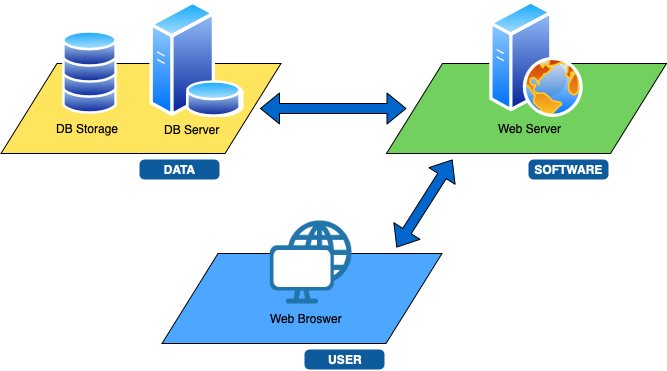
\includegraphics[width=0.85\linewidth]{image/hardware_COMPLETE.png}
    \caption{Overall view of bike4share architecture}
    \label{fig:arch}
\end{figure}

\subsubsection{Parallelism}
“bike4share” must support parallel operations coming from both user and technician on the same database.

\subsection{Assumptions and Dependencies}
\begin{itemize}
    \item Non registered user must have a smartphone or a computer with internet connection available to exploit the “bike4share” services;
    \item Registered user needs a smartphone or a computer with internet connection and active GPS in order to use the premium functions available on the application, e.g. localisation function;
    \item Non registered technician must have a smartphone or a computer with internet connection available to register on the application, the secret key provided by the head of the system and then access the devoted section;
    \item Registered technician is required to have a smartphone or a computer with internet connection in order to access the devoted section of the application;
\end{itemize}

\section{Specific Requirements}
In this chapter is presented a full list of the requirements and the associated use cases.\\It is divided in two subchapters, one devoted to the specifications about the design constraints, such as standards compliance and hardware limitations,and the second one is focused on the software system attributes (i.e. reliability, availability, security, maintainability and portability).

\subsection{External Interface Requirements}
In the following section will be describe in detail how the different interfaces are designed and represented in the b4s web application.
\subsubsection{User Interfaces}
There are different kind of interfaces because in the "b4s" application there are different kind of users, so for any of this different categories there will be more or less functionality visible directly from the interfaces.\\
At the beginning every users will see the same homepage as shown in Figure \ref{fig:homepage}\\
\begin{figure}[H]
    \centering
    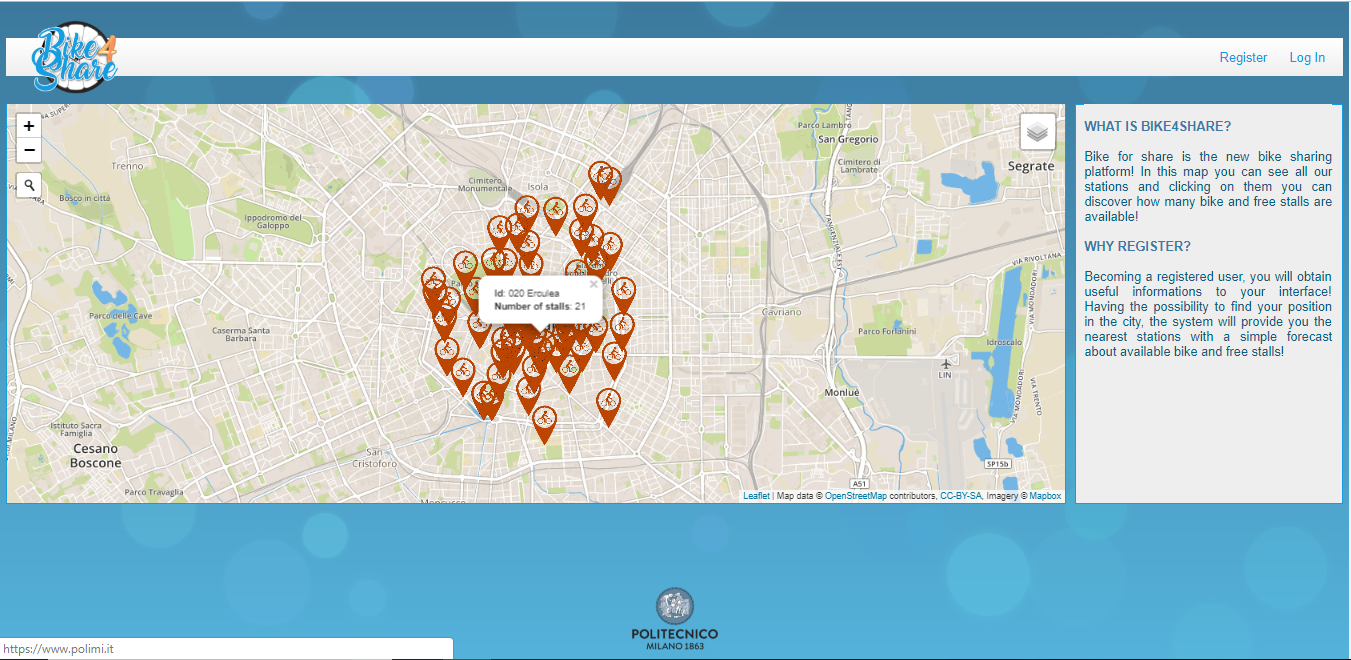
\includegraphics[width=0.75\linewidth]{image/all.PNG}
    \caption{"bike4share" common users interface}
    \label{fig:homepage}
\end{figure}

3.1.1.1 USE CASE:Log-In

In this interface the user is registered yet so it's sufficient to follow the log in procedure and compile the requested fields Figure \ref{fig:log-in 2}
\begin{figure}[h]
    \centering
    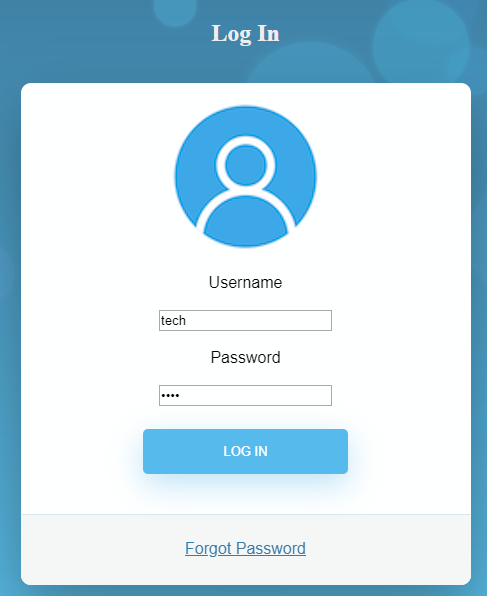
\includegraphics[width=0.35\linewidth]{image/log_in.PNG}
    \caption{"bike4share" common users interface}
    \label{fig:log-in 2}
\end{figure}

\subsubsection{Hardware Interfaces}
Bike4share requires the use of a machine with an internet connection with a modern web browser.
The system must be able to acquire the correct position of the user, therefore the used device must have the possibility to locate itself (e.g. with a GPS services).
\subsubsection{Software Interfaces}
The system is developed both on the front-end and back-end side using the following programming, markup and representation languages:
\begin{itemize}
\item HTML: front end;
\item Javascript: front end;
\item CSS: front end;
\item JSON: front end/back end;
\item Python: back end;
\item SQL: database management;
\end{itemize}
\subsubsection{Communication Interfaces}
Client and server have at their disposal the port 5000 to communicate using HTTP protocol.

\subsection{Functional Requirements}
It is possible to define different type of users, in particular in this document the Log-In case, the Registration case, the Forgot Password case,the Data Visualization (NO PREMIUM) case, the Data Visualization (PREMIUM) case, the Registration of the Technician case, and the Technician Analysis case are shown in their details.

\subsubsection{\textbf{USE CASE}: Log-In}
\begin{enumerate}
\item Participating actors: 
\begin{itemize}
    \item registered user
    \item WebApp
\end{itemize}
\item Entry Condition: 
\begin{itemize}
    \item user wants to access to premium functions (so have to log in)
\end{itemize}
\item Flow of events: 
\begin{itemize}
    \item user enters in the page and puts the username
    \item user inserts also the password
\end{itemize}
\item Exit Condition: 
\begin{itemize}
    \item user is logged in the WebApp
\end{itemize}
\item Exceptions
\begin{itemize}
    \item the username doesn’t exist so a message is shown on the log in page
    \item the password is wrong so a message is shown on the log in page
    \item the password is forgotten so the user can send a request for the password recovery
\end{itemize}
\end{enumerate}

Scenario 1: “bike4share” Log-In \\
Mario needs a bike to go back from his position to his home near to Parco Sempione. He decides to open the “bike4share” WebApp in order to know if there are some bike stalls available near to his position.\\ 
Mario is registered yet so he has to insert his username and his password, in this way he can access to the PREMIUM FUNCTION.\\ 
He is asked to allow the application to use his position and after that he can check the bike stalls distribution on the map. \\
If Mario doesn’t want to allow the usage of his position or if this feature is not available for his system he can insert directly the address and the list of the station will appear on the screen.\\ Now Mario can go by foot to the nearest stalls and finally come back home riding a bike.

\subsubsection{\textbf{USE CASE}: Registration}
\begin{enumerate}
\item Participating actors: 
\begin{itemize}
    \item new user
    \item WebApp
\end{itemize}
\item Entry Condition: 
\begin{itemize}
    \item new users want to register in order to be able to use the Premium Functionalities
\end{itemize}
\item Flow of events: 
\begin{itemize}
    \item new users have to sign in
    \item new users have to insert their e-mail
    \item new users can set an username
    \item new users can set a password
\end{itemize}
\item Exit Condition: 
\begin{itemize}
    \item new users are registered
\end{itemize}
\item Exceptions
\begin{itemize}
    \item the username is already used so a message is shown on the registration page
    \item the format of the mail is wrong so the system requires to correct it and insert a valid one.
\end{itemize}
\end{enumerate}

Scenario 2: “bike4share” Registration \\
Luca wants to take the train starting from the Cadorna railway station at 13.00 p.m. but he knows that he is late and he can’t arrive in time if he goes by foot.\\ Fortunately he works in L.go Greppi near a bike stall so one of his colleagues suggest him to use the “bike4share” WebApp in order to reach the station by bike. Luca tries to use the “bike4share” WebApp in order to discover the list of the stalls near the Cadorna railway station where he could left the bike taken from the L.go Greppi bike stall.\\ 
He doesn’t have so much time and the manual research of his position offered by the BASIC FUNCTIONS of “bike4share” isn’t enough so he needs to access to the PREMIUM FUNCTIONS.
He tries to access directly to the “bike4share” WebApp PREMIUM FUNCTION but the user name doesn’t exist so a message is shown on the log in page 
As new user Luca has to sign in by compiling the form with his correct format e-mail, an user name and a password. 
If the user name that Luca has inserted is chosen yet a message is shown and he has to change the previous chosen name, otherwise the registration is successfully completed.
Now Luca can access to the the “bike4share” WebApp PREMIUM FUNCTION and check the stalls’ list near the Cadorna railway station.

\subsubsection{\textbf{USE CASE}: Forgot Password}
\begin{enumerate}
\item Participating actors: 
\begin{itemize}
    \item user
    \item WebApp
\end{itemize}
\item Entry Condition: 
\begin{itemize}
    \item user forgot the password and wants to restore it
\end{itemize}
\item Flow of events: 
\begin{itemize}
    \item users have to put the username 
    \item users have to put the e-mail associated to the account 
    \item the system sends back the old password using the user e-mail
\end{itemize}
\item Exit Condition: 
\begin{itemize}
    \item user receive by mail a random code that can be used to set the new password
\end{itemize}
\item Exceptions
\begin{itemize}
    \item the users don’t remember anything about the previous registration so it is necessary to do again the registration processes
\end{itemize}
\end{enumerate}

Scenario 3: “bike4share” Forgotten Password \\
Lucy bought a ticket to go to the cinema tonight for a new Marvel’s film.\\ She decides to go with the train but the show finishes at midnight so there won’t be the trains for the return.\\ 
She wanted to save money because she has already spent a lot for the show ticket so instead of booking a taxi she tries to open the “b4sh” WebApp from the internet cafè near the cinema.\\Lucy can’t remember the password of her account but she still need to come back home and so she wants to restore her password.\\ The system requires to insert the e-mail address associated to the account and at this point the system can send an e-mail that deliver to the user a random code that will allow the setting of a new password to the set\_new\_password html page. \\ At this point Lucy can walk to the chosen bike stall and she finds another girls that is trying to remember her credentials but unfortunately this girl can’t remember anything of the previous registration so she has to do again the registration process.\\Lucy helps her to find another stall near her house and at the end they both can pick up a bike and came back home.


\subsubsection{\textbf{USE CASE}: Data Visualization (BASIC FUNCTION)}
\begin{enumerate}
\item Participating actors: 
\begin{itemize}
    \item user not registered
    \item WebApp
    \item map applications as OpenStreetMap, Mapbox Satellite and Mapbox Street 
\end{itemize}
\item Entry Condition: 
\begin{itemize}
    \item user wants to see on a map how many stalls there are  for each station.
\end{itemize}
\item Flow of events: 
\begin{itemize}
    \item user manually checks in the map where the stations are and the numbers of stalls.
\end{itemize}
\item Exit Condition: 
\begin{itemize}
    \item The user has finished to look at the number of stalls and exits from the application. 
    \item the user want to access better functionalities and decides to make the registration procedure
\end{itemize}
\item Exceptions
\begin{itemize}
    \item if the localisation doesn’t work the logged user can insert the address and find the position
    \item maps providers crash
    \item server doesn’t work
\end{itemize}
\end{enumerate}

Scenario 4: “bike4share” Data Visualization (BASIC FUNCTION) \\
Max is a student and he has to go to the university but in the morning there’s an underground line services strike so he wants to see on the map how many bikes and how many stalls are available near Centrale underground station, where he is forced to stopped, and near his university in Piazza Leonardo which he has to reach.\\ 
Thanks to “bike4share” WebApp BASICS FUNCTION he can manually check on the map that there are 2 bike stalls near the underground station and many different bikes available but there aren’t any stalls near Piazza Leonardo so he close the application and maybe he has to find another way to reach the university.


\subsubsection{\textbf{USE CASE}: Data Visualization (PREMIUM FUNCTION)}
\begin{enumerate}
\item Participating actors: 
\begin{itemize}
    \item user registered
    \item WebApp
    \item map applications as OpenStreetMap, Mapbox  Satellite and Mapbox Street 
        \item Bike Data (API database)
\end{itemize}
\item Entry Condition: 
\begin{itemize}
    \item user, considering his position, wants to see on a map how many bikes and how many stalls are available for the nearest station and for all the other ones
\end{itemize}
\item Flow of events: 
\begin{itemize}
    \item user, depending on his position, checks in the map where are the stations and the number of free bikes that are available in this place
    \item user logged in the system and access to Premium Functions 
\end{itemize}
\item Exit Condition: 
\begin{itemize}
    \item If there is availability of bikes in the interested area at this time the user can successfully go to the bike station, otherwise the user closes the application
\end{itemize}
\item Exceptions
\begin{itemize}
    \item localisation doesn’t work so logged user can insert the address and find the position or add a point in his position
    \item user forgets the password, recovery password procedure is needed
    \item maps providers crash
    \item server doesn’t work
\end{itemize}
\end{enumerate}

Scenario 5: “bike4share” Data Visualisation (PREMIUM FUNCTION) \\
Mary wants to invite some of her friends to Parco Sempione in order to spend a funny day together by riding the bikes and to escape from the hottest day of the season, 
She decides to check on “bike4share” WebApp, considering their positions, how many stalls and how many bikes are available in real time for the nearest station of her house and for all the other stations near her friends and Parco Sempione; she can check both looking directly on the map or, if the GPS system does not work, she can insert the address and find the position.
Mary as registered user is logged in the system and she can access to PREMIUM FUNCTIONS that allow her to access to a list of available/occupied stalls  in order to plan a perfect day for her friends.

\subsubsection{\textbf{USE CASE}: Registration of the Technician}
\begin{enumerate}
\item Participating actors: 
\begin{itemize}
    \item new user
    \item WebApp
\end{itemize}
\item Entry Condition: 
\begin{itemize}
    \item Technician register for the first time
\end{itemize}
\item Flow of events: 
\begin{itemize}
    \item technician receives a secret-key by the master of the service
    \item technician inserts the secret-key
    \item technician can set a password
\end{itemize}
\item Exit Condition: 
\begin{itemize}
    \item technician is registered 
\end{itemize}
\item Exceptions
\begin{itemize}
    \item the username is already used so a message is shown on the registration page
    \item the e-mail is already used so a message is shown on the registration page
    \item the secret key is already used so a message is shown on the registration page
\end{itemize}
\end{enumerate}

Scenario 6:  “bike4share” Registration of the Technician \\
Orazio is a new technician that is been assigned to the “bike4share” WebApp data management and data analysis and he must register himself for the first time.\\ 
Orazio has received a fixed username by e-mail from the system and he logs in for the first time with the given username, after that he has to compile the appearing form with his e-mail address and he has to set a password.\\
At the end of the procedure if the e-mail address is formally correct the new technician is successfully registered otherwise an error is shown and the system requires to insert another valid e-mail address. 


\subsubsection{\textbf{USE CASE}: Technician Analysis}
\begin{enumerate}
\item Participating actors: 
\begin{itemize}
    \item technician
    \item map applications as OpenStreetMap, Mapbox, Leaflet
    \item Bike Data (API database)
\end{itemize}
\item Entry Condition: 
\begin{itemize}
    \item technician wants to analyse the distribution of the bike stations and study their trend
\end{itemize}
\item Flow of events: 
\begin{itemize}
    \item technician logs in the system to access to a private section
    \item then technician can check the trend of a bike station in real time and the trend during a time span
\end{itemize}
\item Exit Condition: 
\begin{itemize}
    \item technician wants to stop the analysis
\end{itemize}
\item Exceptions
\begin{itemize}
    \item user forgets the password, so the service for forgot password can be activated
    \item maps providers crash
    \item server doesn’t work
\end{itemize}
\end{enumerate}

Scenario 7: “bike4share” Technician Analysis \\
Clara is an expert technician that wants to analyse the distribution of the bike station and study their trend in order to obtain more information related to the usage of the services offered by the “b4s” system WebApp for her client.\\
She has to logs in the system and make the access to a private section, reserved only for the technicians, where Clara can check the trend of a specific bike station in real time or a time span in which she is interested in.\\ For example she can check if during the lunch time there are enough bikes available in the stall of P.za S.Ambrogio, near the university, in this way she can consider if it’s better to increase the number of bikes in that station or not in order to be able to offer a better service.
At the end of her analysis Clara can close the application and shows to her bosses the results that she has obtained.
If some technician forgets the credentials it is possible to activate the “Forgot Password” service as it is described in the Scenario 3: “bike4share” Forgotten Password.

\subsection{Performance Requirements}
The system is expected to operate with a great number of users simultaneously. This number is not fixed at the time being, but the system should be flexible enough to adapt itself to the number of requests.
\subsection{Design Constraints}
PostgresSQL is used in order to manage the databases
Python is used in order to perform the outputs using the available libraries. 
Libraries as Shapely, Padas and Geopandas are used in order to build the map and to manage a background map with the entities that we want to represent.
Libraries as Numpy, Seaborn and Bokeh are used for the visualisation of the statistics. 
\subsubsection{Standards compliance} The web application runs on every personal computer independently of the OS (it works on both Windows and MacOS). It requires an internet connection and an active localization service.  
\subsubsection{Any other constraint}
After the login phase, the user must agree to give Bike4share the permission to track his/her position. 
Email addresses will not be used for commercial purposes. 
\subsection{Software System Attributes}
\subsubsection{Reliability}
The application must be available 24/7, since the bike sharing service is always active.
\subsubsection{Availability} 
In order to achieve the highest possible availability level (at least 99.99 \%\\ of the time) the server must belong to a collection servers. In this way, even if a single machine fails the others will still work and keep the system up.
\subsubsection{Security}
Security is not the main issue of the application, but it’s essential to guarantee that user’s passwords are stored and encrypted. Finally, the system must guarantee that only registered users can have access to the application’s premium feature and that only technicians can visualize the statistics.

\subsubsection{Maintainability}
Since the architecture can support an easy evolution of the software and the adding of new features and options (taking in consideration the users’ feedback), the development requires the use of an object oriented language to make use of classes and therefore to create a more readable code.
\subsubsection{Portability}
The system is developed to reach any browser. So it must be available on several OS and on any browser (e.g. Google Chrome, Mozilla Firefox).

% \section{Appendices}

\end{document}
